% Instructions from Impact:
% Slide deck (3 slides) in PDF format:
%    Slide 1 (Introduction): Who you are and a summary of the project,
%    emphasizing need and impact
%    Slide 2 (Objectives/Outcomes): SMART (Specific, Measurable, Achievable,
%    Relevant, Time-Bound) goals for the project
%    Slide 3 (Budget): Outlining how the grant money will be used

\documentclass[12pt]{beamer}
\setbeamertemplate{navigation symbols}{}
\usepackage{mathtools}
\usepackage{paralist}
\usepackage{graphicx}
\usetheme{default}
\usefonttheme{serif}
\begin{document}

\begin{frame}[c]{Introduction}

\textbf{Project Frozone} involves:

\small
\begin{compactitem}
\item Stephen Davies (professor of Computer Science \& Data Science)
\item Bethanie Hackett (Computer Science \& Political Science senior)
\item Garrett McKenzie (Computer Science \& Data Science junior)
\item Laur Rider (Computer Science \& English junior)
\end{compactitem}

\bigskip
\begin{columns}[c,onlytextwidth]
  \begin{column}{0.82\textwidth}
    Our goal is to determine whether \textbf{AI chatbots} can be deployed to help \textbf{mitigate political polarization} in a society.
  \end{column}

  \begin{column}{0.18\textwidth}
    \centering
    
\includegraphics[width=\linewidth]{frozone.png}
  \end{column}
\end{columns}

\bigskip
We're training a \textbf{Large Language Model} (LLM) called ``\textbf{Frobot}'' to detect instances of \textbf{misinformation}, \textbf{toxic speech}, and \textbf{entrenched bias} when they appear in online political conversation, and to \textbf{counteract} those elements with its responses.

\end{frame}

\begin{frame}[c]{Objectives/Outcomes}

\small
We plan to evaluate Frobot in two ways (by \textbf{May 2027}):
\footnotesize

\noindent
\begin{minipage}{0.25\textwidth}
    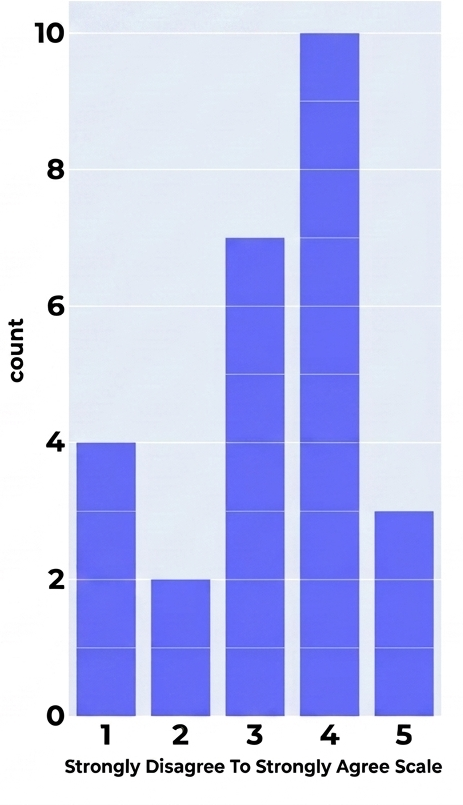
\includegraphics[width=0.297\textheight]{image_b.png}
\end{minipage}
\begin{minipage}{0.65\textwidth}
    \textbf{Firstly, a chatroom}! The Frobot is being deployed to a chatroom with human participants who will chat with \textbf{Frobot}, and other vanilla bots, pretending to be humans. In addition, participants will complete Surveys, one of which is graphed to the right showing which participants believed \textbf{Frobot} helped to make the discussion \textbf{More Productive}.
\end{minipage}%
\vspace{-0.85cm}
\begin{minipage}{0.5\textwidth}
    \textbf{Secondly, a simulation!} The Frobot will be deployed into a large \textbf{artificial social network} where each participant is a bot trained to act like a real person. Using bots as independent actors in the simulation is known as \textbf{LLM Backed Agent Based Modeling}.
\end{minipage}
\begin{minipage}{0.3\textwidth}
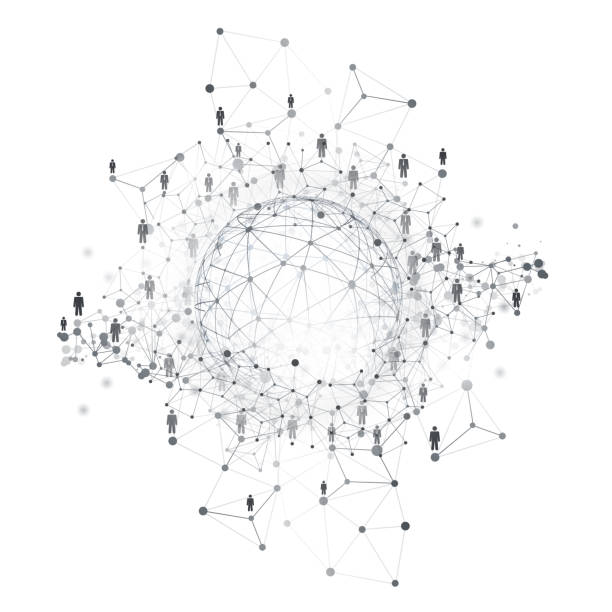
\includegraphics[width=0.6\textheight,height=0.5\textheight]{network image.jpg}
\end{minipage}

\end{frame}

\begin{frame}[c]{Budget}

\small
We seek funding for two things:

\begin{enumerate}
\itemsep.5em
\footnotesize
\item \textsl{Cloud compute time and storage space to train Frobot.} Training LLMs on large amounts of text data is expensive. We plan to use the Google Gemini and Vertex AI suite of tools, at an estimated cost of \textbf{\$1500}.

\item \textsl{Computational power to simulate the ABM.} Analyzing the behavior of an ABM requires running it a large number of times, both to ``even out'' the randomness of each individual trial, and also in order to vary the simulation's inputs to discover how various parameter settings influence the aggregate results. We will use Google Virtual Machines to carry out these resource-heavy computations, and estimate \textbf{\$1000} for this.

\end{enumerate}

\normalsize
Summary:
\begin{compactenum}
\item Training resources: \$1500
\item Simulation resources: \$1000
\end{compactenum}
\begin{compactitem}
\item \textbf{Total funding request: \$2500}
\end{compactitem}

\end{frame}

\end{document}